\section{Diseinua}

\subsection{Informazio sistemak}
\label{sec:dinf}
\subsubsection{ITIL prozesuak}
Inzidentziak nola jasoko diren definitu aurretik, beharrezkoa da definitzea enpresak berak nola jokatuko duen inzidentzia bat jasotzerakoan, hortik gero plano praktikora jaitsi eta aplikazioa nola garatuko den pentsatuz. Baina, hori egin baino lehen, nahitaezkoa da IT departamentuaren egitura definitzea, hau da, departamentua nortzuk osatuko duten. Osaketa hori egiteko, 14 pertsona eskuragarri izango ditugula uste da.

Jarraian zerrendaturiko dira IT departamentuak kudeatu beharko lituzkeen zerbitzuak, heziketa arloko enpresa bat dela suposatuz:

\begin{itemize}
 \item Moodle
 \item Webgunea
 \item Web zerbitzuak (idazkaritza birtuala, intranet)
 \item E-posta zerbitzuak
 \item Erabiltzaileen kudeaketa
 \item Baliabideen kontrola (nominak, ERP-a)
 \item Datu-base desberdinen kudeaketa
 \item Sarearen kudeaketa (barne-sarea, interneterako sarbidea)
 \item Ordenagailu pertsonalen kudeaketa (instalazioak e.a.)
 \item Datuen segurtasuna kudeatu
\end{itemize}

Ikusita zerbitzuak zeintzuk diren, ikusi beharko da, gure bezeroei (enpresako gainerako zatia) eskaintzen diegun zerbitzu hauen arabera, nola egongo den banatuta gure departamentua, zerbitzu hauen garrantziaren eta eskatutako lanaren arabera. Era berean, departamentuaren muina da erabiltzaileen eskariak aztertu eta konpontzea, baita funtzionalitate berriak ahal den heinean txertatzea, enpresaren eguneroko jarduna ahalik eta gutxien oztopatu eta kontrara, berau bultzatzeko.

\ref{fig:egitura} irudian agertzen den moduan banatu dugu gure balizko departamentua:

\begin{figure}
\centering
   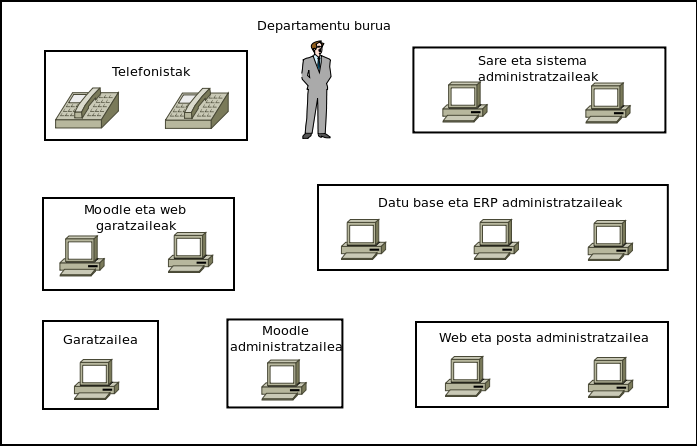
\includegraphics[scale=0.5]{irudiak/cau.png}
   % Laster-markak gehitzeko menua
   \caption{IT departamentuaren egitura}
   \label{fig:egitura}
\end{figure}


\begin{description}
 \item [Departamentu-burua] (pertsona bat). Izenak dioen moduan, gure IT departamentua eta beraz, Service Desk-aren burua izango litzatekeen pertsona da, formazio tekniko zein kudeaketarakoa duen pertsona litzateke berau, erabaki estrategikoak hartu eta azken hitza esateko ahalmena izateko. Era berean, gure departamentua eta gainerakoen arteko zubia litzateke, enpresako erabakietan informazio teknologien esparruan aholkatuz, edota soluzio berriak eskainiz. Ez luke parte hartuko zerbitzuen kudeaketa zuzenean, baina zerbitzuen araberako baliabideak lortzeko gaitasuna luke eta departamentuaren martxa on edo txarraren arduradun edo erantzule izango litzateke.

 \item [Hartzaileak] Bi pertsona. Arduraduna maila administratibo batean enpresarekin dugun lotura den bezala, hartzaileak, egunerokotasunean gertatzen diren gora-beheretzako kontaktuak lirateke. Zubia lirateke, beraz, gora-behera duten pertsonen eta gora-behera hori konpontzeko gai diren pertsonen artean. Arazoa konpontzeko erraza baldin bada edota askotan errepikatutakoa, eurak izango lirateke zuzenean erabiltzaileari eskaera konponduko lioketenak. Beraiek ikusiko lukete ea inzidentzia berriak dauden edo ez.

\item [Moodle eta Web garatzaileak] bi lirateke eta euren lana, Moodle-i funtzionalitate berriak gehitu edota web aplikazioak garatzea/eguneratzea litzateke, esate baterako, enpresako intranet sarean jartzeko.

\item [Garatzaile bat] Honek ere, aurrekoek bezala, aplikazioak garatuko lituzke, baina ez web ingurune baterako, baizik eta datu-base bateko interfazea, kalkuluak egiteko zenbait aplikazio... garatuko lituzke.

\item [Moodle administratzailea] Moodle zerbitzua behar bezala dabilela ziurtatuko duen pertsona da, erabiltzaileak alta eta baja emateaz gain. Bera litzateke arduraduna zerbitzua, gero ezarriko diren baldintzen pean mantentzeko.  

\item [Bi Web eta posta administratzaile] Hauek, webguneak, garaturiko web aplikazioak eta posta zerbitzua mantenduko luketen pertsonak dira, erabiltzaileentzat ahalik eta eskuragarrien jarriaz.

\item [Bi Sistema eta sare administratzaile] Sistema (zerbitzariak, erabiltzaileen ekipoak...) eta sarea kudeatuko luketen pertsonak dira.

\item [Hiru datu-base eta ERP administratzaile] Horietatik bi arduratuko lirateke ERPa kudeatzeaz eta bestea datu-baseko administratzaile modura. ERPko administratzaileetariko bat, datu-baseko administratzaile ere izan daiteke, besteari lagundu eta zerbitzu hobe bat eman ahal izateko.
\end{description}

Behin departamentua osaturik, bi hartzaile eta hainbat adituk osatuko luketela ikusirik, inzidentzia baten aurrean nola jokatuko litzatekeen definitu behar da, ITIL liburuetan azaltzen den modura. Gurean, \ref{fig:inzidentzia}. irudian ikus daiteke nola jokatuko den inzidentzia baten aurrean. Bertan,\textit{Arazoen kudeaketa} izeneko hitzak agertzen dira, baina hori askoz ere hedadura handiagoa duen gaia da eta lan honetako zioa baino askoz harago doa. Lan honetan suposatuko da, inzidentzia guztiak atoan konpondu edo bestela workaround (momentuko konponketa), zerbitzuaren aldaketa sakonak beste era batera landu beharreko gaia litzateke.

\begin{figure}
   \centering
   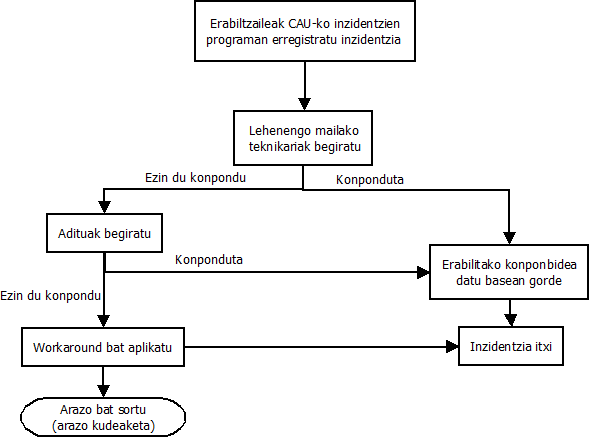
\includegraphics[scale=0.4]{irudiak/gestionInzidentzia.png}
   % Laster-markak gehitzeko menua
   \caption{Inzidentzien kudeaketa}
   \label{fig:inzidentzia}
\end{figure}

\subsubsection{CMDB}
Behin enpresan nola jokatuko den definiturik dagoela, behar-beharrezkoa da dokumentaturik izatea zeintzuk diren inzidentziekin loturik egongo diren elementuak, hau da, enpresako IT aktiboak. Beharrezkoa da ondo gordeta izatea aktibo bakoitza zer den, zein atributu dituen eta zein den aktibo horren jabe edo arduradua. Horretarako tresna, CMDB-a da.

CMDB (\textit{Configuration management database, Konfigurazioaren kudeaketarako datu-basea}) delakoa da inzidentziak gordetzeko web aplikazioaren muina. Bertan daude gordeta, IT teknologiekin loturiko enpresako aktibo guztiak (CI edo konfigurazio item-ak deritzena). \ref{fig:cmdb}. irudian ikus daiteke zein den CMDB-aren egitura. Aktibo gehienak taula berean daude jarrita, kodeak esleitzerako orduan erraztasuna izateko. Era berean, asmo horrekin garaturiko funtzioen bitartez sartuko dira datuak datu-basean, erabiltzailearentzat taulako NULL balio guztiak guztiz gardenak izango direlarik.

\begin{figure}
\centering
   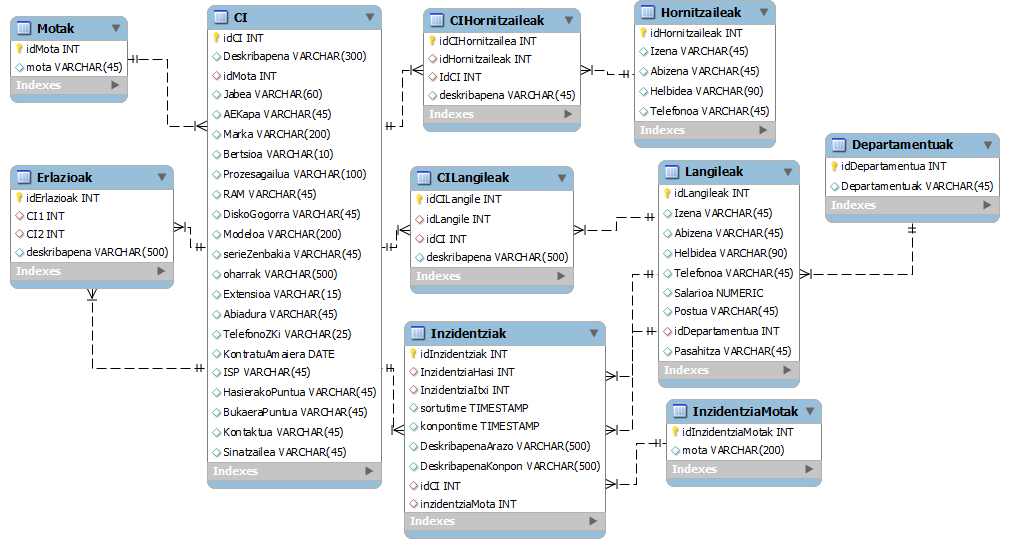
\includegraphics[scale=0.4]{irudiak/cmdb.png}
   % Laster-markak gehitzeko menua
   \caption{CMDB-aren eredu erlazionala}
   \label{fig:cmdb}
\end{figure}

\ref{fig:cmdb}. irudian ikus daitekeenez, inzidentziak gordetzerako orduan, inzidentzia kodea, inzidentzia zabaldu duen langilearen kodea, inzidentzia itxi duen langilearen kodea, inzidentzia hasi zen momentua, bukatutako momentua, inzidentziaren deskribapen laburra, konponketaren inzidentzia laburra, inplikaturiko konfigurazio itemaren kodea eta, azkenik, zein inzidentzia mota litzatekeen, motak, beste taula batean egongo lirateke, kategorizatuta. Era honetan, inzidentziaren inguruko datu guztiak gorde ahal izango lirateke, bertan.

\subsubsection{Inzidentzien web aplikazioa}
\label{sec:webapdis}
Erabiltzaileak web orrira sartzean izena eta pasahitza sartu beharko dute (datubasean hash baten bitartez egongo direlarik gordeta), gure enpresan lana egiten dutela ziurtatzeko. Behin sisteman logeatuta, inzidentziak sortzeko aukera, edo enpresako CI(configuration item) ezberdinak ikusteko aukera izango dute. Inzidentzia bat zabaltzerako orduan, langileek beraien kodea eta intzidentzia infektatzen dion itemaren kodea sartu beharko du, deskribapen batekin eta intzidentzia mota bat aukeratuz. 

IT departamentuko langileak badira ordea, honetaz gain jendeak zabalduriko intzidentziak ikusteko edota ixteko gaitasuna ere izango dute. Inzidentzia bat ixtean intzidentzia hori konpontzeko bete behar izan diren pausuak idatzi beharko ditu langileak, dokumentazio eta erreferentzia modura gordeta izateko.

\subsection{Metodologia}
\subsubsection{Kodifikazio manuala}
\ref{sec:webapdis} atalean azaldu den aplikazioa garatzen hasi baino lehen, beharrezkoa da jakitea aplikazioa \textit{nola} garatuko den. Ez funtzionalitate aldetik, horiek jada definiturik baitaude, baizik eta kode aldetik nola egongo den eginda. Era honetan lortzen dena da, kodearen estiloan uniformetasun bat bermatzea, egingo diren berrikuspenak erraztu (programatzaile bakoitzaren programazio-estiloak inpaktu txikiagoa izango baitu eta komentatuta egongo baita), bertsio berriak egitea errazteko (kodifikazio manualak, kodea berriztagarria izateko irizpideak lantzen baditu, bederen). Finean, kode eraginkorragoa eta ikuspegi profesionalagoa emango diona egitea dugu helburu. Irakurleak nahi izanez gero \ref{sec:kodman} eranskinean du ikusgai manuala osorik.

\subsubsection{Bertsio-kontrola}
Behin kodea nola idatziko dugun definitu dugula, beharrezkoa da era eraginkorrean kode hori garatzeko bitartekoak izatea. Hainbat pertsonen artean kodea garatuko delarik (era eraginkorrean espero da, horretarako sortu baita kodifikazio manuala), beharrezkoa da bakoitzak izango duen bertsioa azkena izatea, integraziorako aldaketak ez egoteko eta garatzaile guztiek funtzionalitate aldetik bertsiorik osoena izateko. 

Gainera, funtzionalitate oso interesgarriak eskaintzen dituzte.

\begin{itemize}
 \item Kudeatu beharreko kodearen biltegiratzea.
 \item Kodeari aldaketak egitea ahalbidetzea.
 \item Eginiko aldaketa guztiak erregistratzea.
\end{itemize}

Beraz, ez da izango beharrezkoa garatzaile guztiek kode osoa izatea euren laneko makinetan, errepositoriotik deskargatu, bertan landu (aldaketa partzialak, fitxategiak gehitu, kendu...) besterik ez baitu egin beharko.  Gainera, ikusi ahal izango da nork egin duen zein aldaketa.

Gure kasuan Git softwarea aukeratu dugu, web zerbitzu bati lotura egonik, beti eskuragarri dago (guk zerbitzari moduan erabiliko geunkeen ordenagailu jakin batean gorde behar izan gabe kodea, baliabideak aurreztuz). Gainera, funtzionalitate gehigarri gisa, bezeroa ere sartu ahalko litzateke web interfaze horretara bere lanaren nondik norakoak nola doazen ikusi ahal izateko (hala nahi izanez gero, noski). Ezingo luke edukirik igo web interfazetik, baina ikusi ahal izango luke berau. \ref{sec:gitinp} atalean azalduko da tresna hau nola erabiltzeari buruzko argibide praktikoak.

Direktorioen estrukturari dagokionez, hiru direktorio nagusi leudeke: bat garapen nagusirako eta beste bi albo lanetarako (datu-baseko datuak eta proiektuaren dokumentazioa). Kasu honetan, direktorio laguntzaileen kasuan, ez luke lagunduko bertsio-kontrola eginez, baizik eta sarean dagoen errepositorioa izanez, fitxategiak gordetzeko.

\subsubsection{Berrikuspenak eta Frogak}
Berrikuspen eta frogen helburua, kodea behin sorturik dagoela ahalik eta arazo gutxien dituela bermatzea da, bai \textit{bug}ak bilatuz zein funtzionalitateak betetzen dituela ikusiz. Berrikuspenen helburua garatzaile batek idatzitako kodea beste garatzaile edo kodea irakurtzeko gai den beste norbaitek, ea bug-ik sortu daitekeen edo egin beharreko funtzionalitateak betetzen dituen garatzaileak sortutako kodea. Gure kasuan, lan-talde txikia izanik, jende desberdinak egindako kodea guk ikus dezakegu, sistematikoki. Aurretik aipaturiko errepositorioan kodea izanda, erraztu egiten du kodea begiratzearen lana. 
 
Frogei dagokionez, bi eratako frogak daude, kutxa beltzekoak eta kutxa zurikoak. Kutxa beltzekoetan ez da kodea begiratzen eta aplikazioak ea espero den moduan jokatzen duen aztertzen da, hau da erabiltzaile normal batek, kode itxiko aplikaziobatean erreportatuko lukeena, gauza jakin bat ezin daitekeela egin aplikazioarekin. Kutxa beltzeko frogen helburua, erabiltzaileak egin ditzakeen pausuak errepikatzea da (funtzionalitateak eskura izanik), erroreak geronek ikusteko, erabiltzailearengana heldu baino lehen.

Kutxa zuriko frogak, jada kodea ikusgai daukagularik egiten dira (hortik izena, gardentasuna-edo erakutsiz) eta kodean dauden balioen arabera egiten dira frogak (String bateko balioak zeintzuk diren ikusirik, balio hori baino handiagoak jarriaz, adibidez edo funtzio bati beste aldagai mota bat pasaz). 

\noindent \textbf{Definituriko frogak}
\noindent \textbf{Kutxa beltzeko frogak}

\begin{itemize}
\item Erabiltzaile izen edo pasahitz oker bat sartu
\item Langile arrunt baten erabiltzaile izen eta pasahitz zuzenak sartu eta aktiboak ikusteko aukeratu
\item Informatikari bat logeatu eta inzidentzia historikoak ikusi
\item Informatikari bat logeatu eta inzidentziak ikusi
\item Informatikari batek inzidentzia berri bat sortu ondoren inzidentziak ikusteko sakatu-
\item Informatikari batek inzidentzia bat itxi eta inzidentziak ikusteko sakatu
\item Informatikari batek inzidentzia bat itxi eta inzidentzia historikoak ikusteko sakatu
\end{itemize}


\noindent \textbf{Kutxa zuriko frogak}
\begin{itemize}
\item Inzidentzia bat sortu eta begiratu inzidentzia berriarentzat kode berri bat sortzen den automatikoki
\item Inzidentzia bat sortu eta begiratu inzidentzia hori sortu den data benetan sortu den dataren berdina den.
\item Inzidentzia bat sortu erabiltzaile batekin eta begiratu ea inzidentzia sortu duen erabiltzailearen kodea benetan inzidentzia sortu duenarena den.
\item Inzidentzia mota berri bat sartu datu basean eta begiratu ea inzidentzia mota berri hori comboboxean agertzen den
\item Aktibo berri bat sartu eta ondoren begiratu aktibo hori agertzen dela.
\item Inzidentzia bat itxi eta begiratu konponduta parametroaren egoera aldatzen den.
\item Inzidentzia bat itxi eta begiratu inzidentzia itxi duen langilearen kodea ongi gordetzen den.
\item Inzidentzia bat itxi eta begiratu inzidentzia itxi den data ongi gordetzen den.
\end{itemize}

\subsection{Segurtasuna}
\label{sec:dsec}
Aipatu bezala, beraz, web aplikazioa sare lokaletik kanpo joango da, baina era berean kanpoko saretik babestuta joango den inguru batean. Inguru horri, DMZ (\textit{DeMilitarized Zone,  zona desmilitarizatua}) deritzo, bi \textit{fronte} ezberdinen arteko mugan baitago, aparteko ingurune batean. Era honetan, bertara sarbidea kontrolatuko duen firewall-aren bitartez, sare lokaletik eta kanpotik, VPN bat erabilita sartu ahal izango da.

\begin{figure}
\centering
   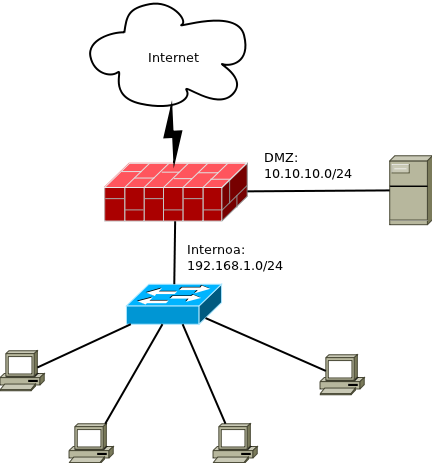
\includegraphics[scale=0.5]{irudiak/sarea.png}
   % Laster-markak gehitzeko menua
   \caption{Sarearen eskema}
   \label{fig:sarea}
\end{figure}

Firewall-ak, horretarako, konexioak baimendu behar ditu, bai sare lokal eta DMZ artean, baita kanpotik datorren VPN bitartezko trafikoa (kanpoko langileak eta batez ere zerbitzu teknikoko enpresa) ere. Beste konexio guztiak deseginez, DMZ horren segurtasuna bermatzen dugu, guk espreski baimentzen ez diogunari sarbidea ukatuz.

Laburbilduz, hauek lirateke Firewall-eko oinarrizko arauak (portuak ez dira esplizituki adierazi, zerbitzu bakarra dagoelako, suposatuko da, zerbitzaria helburu duten paketeak 80. portura joango direla eta erantzunak $>1024$ portuetara).
\bigskip


\begin{tabular}{|c|c|c|c|c|c|}
\hline
 Jatorrizko helbidea & Helburu helbidea & Protokoloa & Flag-ak & Ekintza \\ \hline
 192.168.1.0/24 & 10.10.10.0/24 & http &  & Baimendu \\ \hline 
 10.10.10/24 & 192.168.1.0/24 & http & STB & Baimendu \\ \hline
 192.168.1.0/24 & ANY & http &  & Baimendu \\ \hline
 ANY & 192.168.1.0/24 & http & STB & Baimendu \\ \hline
 220.100.65.98 & 10.10.10/24 & vpn & & Baimendu \\ \hline
 10.10.10/24 & 220.100.65.98 & vpn & STB & Baimendu \\ \hline
 ANY & ANY & ANY & & Ez baimendu \\ \hline
\end{tabular}

Era honetan, zerbitzu teknikoko enpresakoek (zeina 220.100.65.98 helbidea erabiliko luketen), gure enpresakoekin batera kontsultak egin ahal izango lukete sarearen bitartezko VPN trafiko zifratua erabiliz. VPN zerbitzaria, Firewall-eko 10.10.10/24 sareko gateway-ean egongo litzateke eta beste enpresakoak, bertako IP helbidea jakinda, euren VPN bezeroa erabiliz konektatu ahalko lirateke, baina, esan bezala, bakarrik euren enpresako helbidetik.